\section{Pipeline (D.R.)}
\label{sec-pipeline}
Die Pipeline wurde mit der Programmiersprache C\# \cite{billwagner} entwickelt. Den Anfang bildet die Schnittstellenanbindung an die REST-API der Website 
\href{https://www.pegelonline.wsv.de/webservice/ueberblick}{https://www.pegelonline.wsv.de/webservice\\/ueberblick}, 
die eine Möglichkeit bietet, verschiedene Wasserdaten abzurufen. Die Datenpunkte werden in einem JSON-Format bereitgestellt und in der C\#-Applikation
auf eine objektorientierte Struktur gemappt. Anschließend werden die Daten ausgewertet und in einen anderen, objektorientierten Aufbau konvertiert. Diese Konvertierung wird benötigt, 
damit die Objekte entsprechend den Relationen mit dem Entity-Relation-Mapper in eine Postgres-Datenbank geschrieben werden können.
Im letzten Schritt wird die Software über Docker bereitgestellt, weil die Software zusammen mit der Datenbank und dem Frontend 
auf einem Linux-Sever läuft. Außerdem bietet diese Art der Implementierung 
weitere Vorteile, dazu gehören Sicherheit, gute Portabilität und schnelle Softwarelieferzyklen.  
\begin{figure}[H]
    \centering
    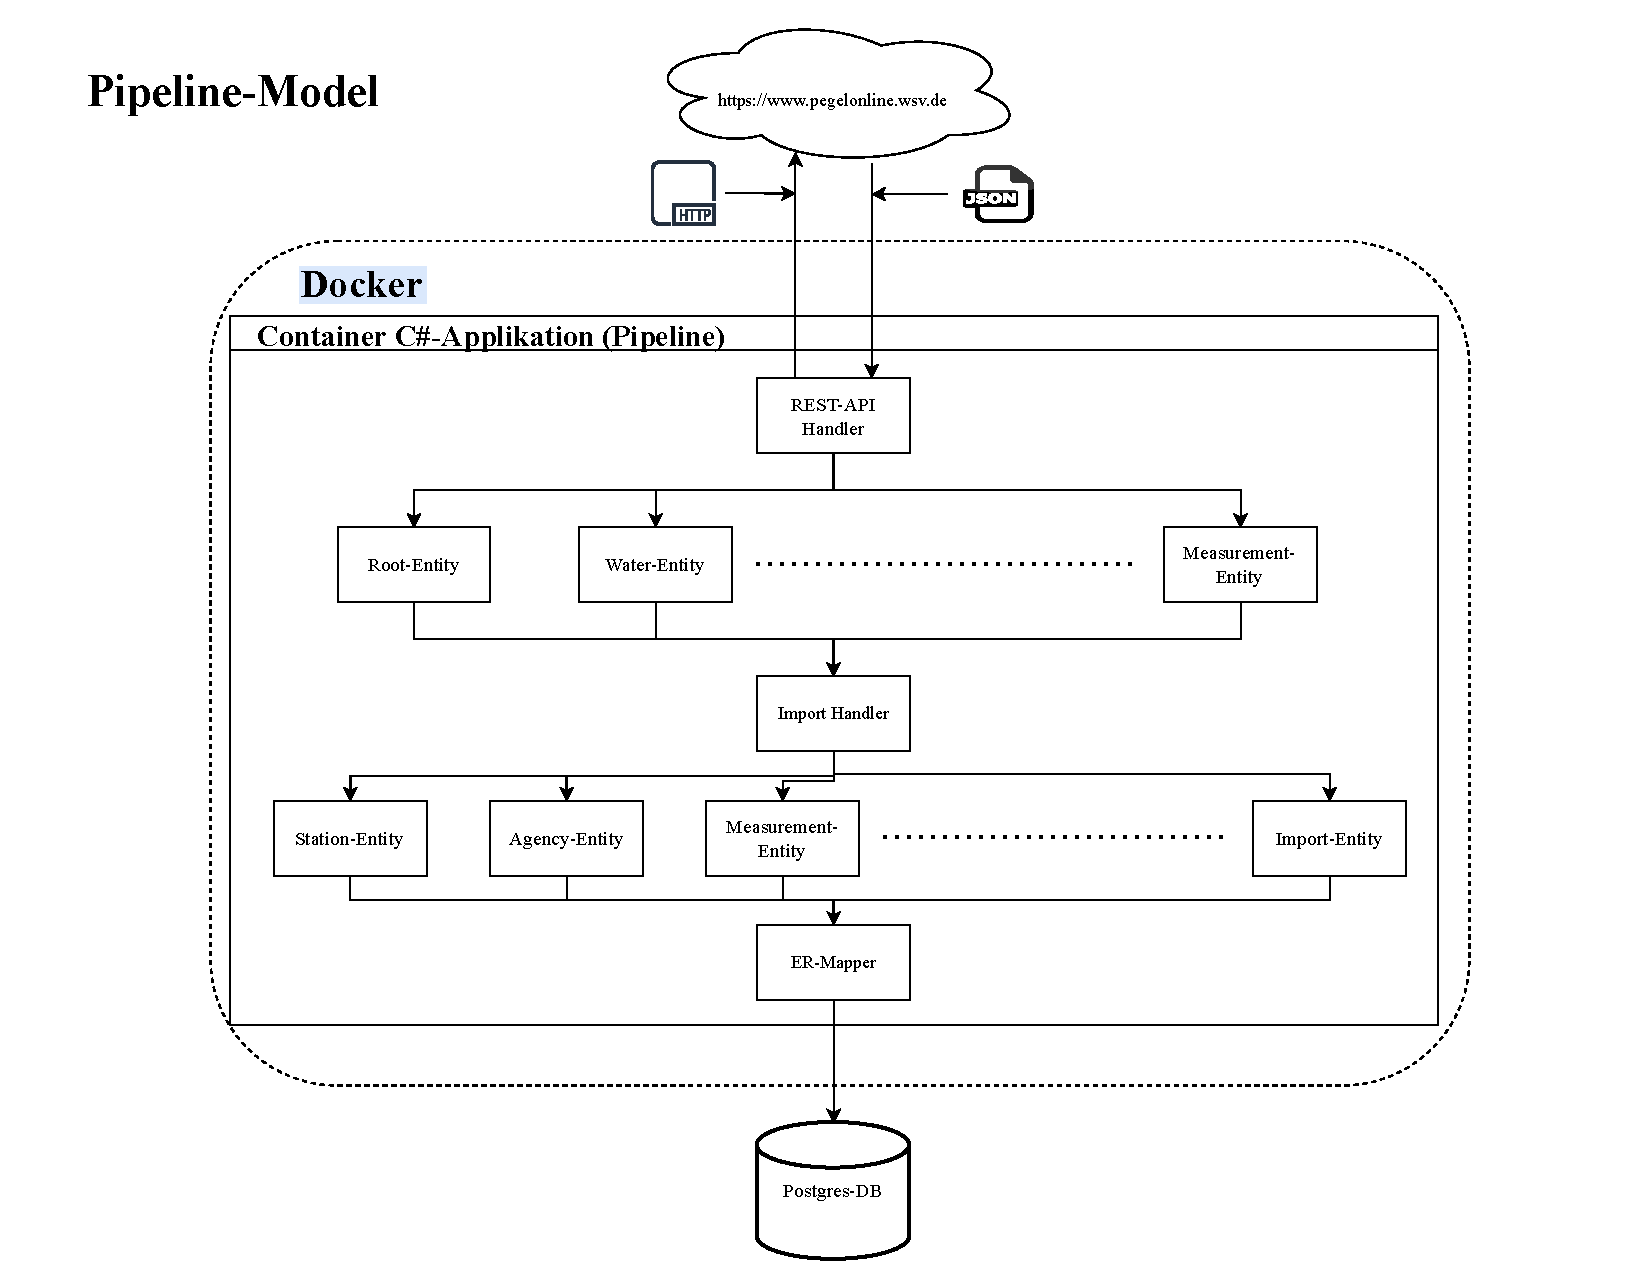
\includegraphics[width=\linewidth]{figures/Pipeline.pdf}
    \label{fig:pipeline}
    \caption{Pipeline Modell}
\end{figure}
\newpage
\subsection{REST-API}
\label{sec-rest-api}
Die Wasserdaten werden zyklisch geladen. Das Zeitintervall lässt sich beim Start der Software über eine Umgebungsvariable einstellen und wurde für dieses Projekt auf 10 Minuten gesetzt. Damit die Daten geladen werden können, 
muss eine Client-Verbindung aufgebaut und ein HTTPS-Request gesendet werden. 
Dieser Request ist parametrisierbar, um die gewünschten Daten in einem bestimmten Format zu erhalten. Für dieses
Projekt wurde auf die stations.json mit folgendem Request zugegriffen: \\
\begin{center}
    \href{https://www.pegelonline.wsv.de/webservices/rest-api/v2/stations.json?includeTimeseries=true&includeCurrentMeasurement=true}{https://www.pegelonline.wsv.de/webservices/rest-api/v2/stations.json?\\includeTimeseries=true\&includeCurrentMeasurement=true}  
\end{center}\vspace{0.5cm}
Die Parameter \textit{includeTimeseries} und \textit{includeCurrentMeasurement} sorgen dafür, dass die aktuellen Werte der Wasserdaten an die entsprechenden Stationen
angehangen werden. Der Aufruf erfolgt in der Applikation über die Klasse \textit{System.Net.Http.HttpClient}, welche den JSON-String entgegennimmt und in die
passende Objektstruktur konvertiert. Die konkrete Implementierung befindet sich im Anhang unter Abbildung \ref{fig:restApi}.

\subsubsection{Aufbau der JSON}
\label{sec-struc-json}
Über den im Abschnitt \ref{sec-rest-api} beschriebenen Request wird der JSON-String abgerufen. Für das Projekt sind alle Daten relevant und sehen folgendermaßen aus:
\begin{itemize}
    \item \textit{uuid - String:} Eindeutige ID der Station.
    \item \textit{number - String:} Eindeutige Nummer jeder Station.
    \item \textit{shortname - String:} Abkürzung des Stationsnamens. Oft identisch zu dem ausgeschriebenen Namen.
    \item \textit{longname - String:} Ausgeschriebener Name der Station.
    \item \textit{km - Float:} Der Kilometerstand innerhalb des Gewässers.
    \item \textit{agency - String:} Die Behörde, die zu der Station und den Messwerten gehört.
    \item \textit{longitude - Float:} Längengrad der Station.
    \item \textit{latitude - Float:} Breitengrad der Station.
    \item \textit{water - Dictionary:} Enthält den ganzen Namen und die Abkürzung des Gewässers.
    \begin{itemize}
        \item \textit{shortname - String:} Abkürzung des Gewässers.
        \item \textit{longname - String:} Ausgeschriebener Name des Gewässers.
    \end{itemize}
    \item \textit{timeseries - List:} Die Liste beinhaltet alle Informationen zu den aktuellen Messwerten.
    \begin{itemize}
        \item \textit{shortname - String:} Abkürzung des Messwertes.
        \item \textit{longname - String:} Ausgeschriebener Name des Messwertes.
        \item \textit{unit - String:} Einheit des gemessenen Wertes.
        \item \textit{equidistance - Int:} Der zyklische Zeitabstand der gemessenen Werte.
        \item \textit{currentMeasurement - Dictionary:} Hier werden alle Informationen zu den sich ändernden Messwerten geliefert.
        \begin{itemize}
            \item \textit{timestamp - String:} Der Zeitpunkt der Messung und die Abweichung zu der UTC-Zeit.
            \item \textit{value - Float:} Aktueller Messwert.
            \item \textit{trend - Int:} Beschreibt, ob der Messwert fällt (-1), gleich bleibt (0) oder steigt (1).
            \item \textit{stateMnwMhw - String:} Setzt den mittleren niedrigsten Wert (Mnw) und den mittleren höchsten Wert (Mhw) in Beziehung. Kommt nur bei Wasserstand-Messwerten vor.
            \item \textit{stateNswHsw - String:} Beschreibt das Verhältnis zwischen dem niedrigsten Schifffahrtswasserstand (Nsw) und dem höchsten Schifffahrtswasserstand (Hsw). Kommt nur bei Wasserstand-Messwerten vor.
        \end{itemize}
        \item \textit{gaugeZero - Dictionary:} Beschreibt die Höhe der Messstation gemessen an einer bestimmten Einheit.
        \begin{itemize}
            \item \textit{unit - String:} Einheit zu der die Höhe gemessen wurde, zum Beispiel Meter über Null.
            \item \textit{value - Float:} Höhe der Messstation.
            \item \textit{validFrom - String:} Jahr, Monat und Tag der Messung.
        \end{itemize}
    \end{itemize}  
\end{itemize}
Ein Ausschnitt aus einer Abfrage befindet sich im Anhang unter der Abbildung \ref{fig:jsonExample}.

\subsubsection{JSON zu Entity}
Der zurückgelieferte JSON-String wird direkt in eine Liste von Root-Objekten durch den HttpClient (Abbildung \ref{fig:restApi}) konvertiert und die Knotentypen werden durch entsprechende Klassen repräsentiert.
Die Attribute sind in den jeweiligen Klassen die Felder. Die Beziehung der Baumstruktur wird durch Felder, welche die erzeugten Objekte der anderen Klassen
halten, berücksichtigt. Die nächste Abbildung stellt die Beziehung zwischen dem JSON-Format und den Klassen 
exemplarisch für Root/Station und Water/Water da.

\begin{figure}[H]
    \centering
    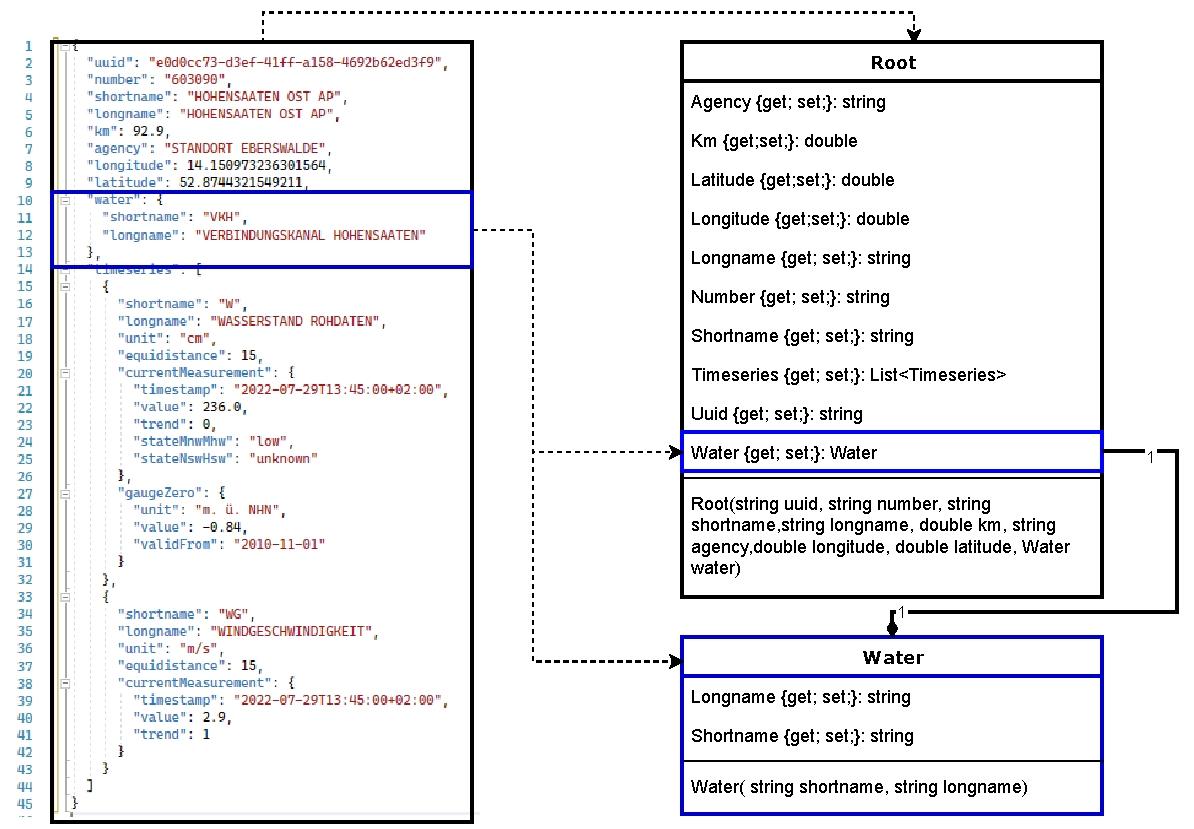
\includegraphics[width=\linewidth]{figures/classDiagramJsonEntities.pdf}
    \label{fig:jsonToEntity}
    \caption{Beispiel: JSON zu Entity}
\end{figure}

\subsection{Datenbankanbindung}
\label{sec-datenbankanbindung}
In diesem Projekt wird die SQL-Datenbank PostgreSQL verwendet. Das Schema (siehe Kapitel \ref{sec-db}) für die Daten wurde nach den Prinzipien der Normalisierung gestaltet. Damit die Objekte im Speicher durch die Software
in ein konsistentes Datenbankformat konvertiert werden können, wird ein Entity-Relation-Mapper benötigt. Weil die Software in C\# entwickelt worden ist, wurde sich für
das EF Core \cite{ajcvickers} von Microsoft entschieden. Das Framework bietet die Möglichkeit, die Datenbank zu modellieren und eine einfache Übersetzung in DML oder DQL basierend auf Listen und
Lambda Ausdrücken. Zum Beispiel wird der folgende Zugriff auf eine Liste direkt in ein SQL-Statement übersetzt:
~\\
\begin{lstlisting}[language={[Sharp]C}, caption={Beispiel: Zugriff auf Listen mit EF Core}, captionpos=b, label={Script}]
    var mem = (from c in dbHandler.DbContext.Stations
                       where c.Uuid == root.Uuid
                       select c).FirstOrDefault();
\end{lstlisting}~\\
Im nächsten Listing befindet sich das aus dem Zugriff übersetze SQL-Statement.
~\\
\begin{lstlisting}[language={[Sharp]C}, caption={Beispiel: Erzeugtes SQL-Statement}, captionpos=b, label={Script}]
    SELECT * FROM "TBL_STATION" WHERE "UUID" = 'Wert in root.Uuid' LIMIT 1
\end{lstlisting}
\subsubsection{Entity Framework}
\label{sec-entity-framework}
Das Datenbankschema wird durch die Klasse \textit{DbContext} und Entity-Klassen, welche logisch zu den Relationen gehören, ermöglicht. In DbContext kann beim Start der Software
festgelegt werden, welche Relationen erzeugt werden, wie die Kardinalitäten zwischen den Relationen sind, wie die Schlüssel aufgeteilt werden und welche Constraints
existieren sollen. In den Entity-Klassen wird der Aufbau der einzelnen Relationen beschrieben.
~\\
\begin{lstlisting}[language={[Sharp]C}, caption={Beispiel: DbContext erstellen von einem Modell}, captionpos=b, label={Script}]
    ...

    protected override void OnConfiguring(DbContextOptionsBuilder optionsBuilder)
    {
        if (!optionsBuilder.IsConfigured)
        {
            optionsBuilder.UseNpgsql(connectionString);
        }
    }
    protected override void OnModelCreating(ModelBuilder modelBuilder)
    {
        modelBuilder.Entity<Station>()
            .HasOne(s => s.Agency)
            .WithMany(c => c.Stations)
            .HasForeignKey(s => s.AgencyForeignKey)
            .OnDelete(DeleteBehavior.Cascade);

        modelBuilder.Entity<Station>()
            .HasOne(s => s.Water)
            .WithMany(c => c.Stations)
            .HasForeignKey(s => s.WaterForeignKey)
            .OnDelete(DeleteBehavior.Cascade);

        modelBuilder.Entity<Measurement>()
           .HasOne(s => s.Station)
           .WithMany(c => c.Measurements)
           .HasForeignKey(s => s.StationForeignKey)
           .OnDelete(DeleteBehavior.Cascade);

        ...
    }
\end{lstlisting}~\\
In der Methode \textit{OnModelCreating} ist exemplarisch das Modellieren von der Relation \textit{TBL\_STATION} (siehe Kapitel \ref{sec-db-modell}) 
durch die Entität \textit{Station} abgebildet. Durch \textit{.HasOne} und \textit{.HasMany} werden die Kardinalitäten dargestellt.
In diesem Modell soll \textit{Agency} n \textit{Station} besitzen und jede \textit{Station} zu einer \textit{Agency} gehören.
Außerdem wird der Fremdschlüssel festgelegt, indem auf das entsprechende Feld in \textit{Agency} verwiesen wird.
Als letztes wird der Constraint erzeugt. Damit werden alle \textit{Stationen}, die zu der \textit{Agency} gehören, entfernt, falls die \textit{Agency} gelöscht wird.
Die Felder der Klassen geben zusammen mit deren Attributen die Spalten der Relationen in der Datenbank wieder.
Außerdem wird durch die Klasse die Relation und deren Namen beschrieben.
~\\
\begin{lstlisting}[language={[Sharp]C}, caption={Beispiel: Felder und Attribute einer Klasse}, captionpos=b, label={Script}]
    ...

    [Table("TBL_MEASUREMENT")]
    public class Measurement : EntityBaseImport
    {
        private int equidistance = -1;
        [Column("EQUIDISTANCE", Order = 8)]
        [Comment("Distance")]
        public int Equidistance
        {
            get
            {
                return equidistance;
            }
            set
            {
                this.equidistance = value;
            }
        }

        private DateTime measurementTimeStamp = DateTime.Now;
        [Column("MEASUREMENT_TIMESTAMP", Order = 9)]
        [Comment("measurement timestamp")]
        public DateTime MeasurementTimeStamp
        {
            get
            {
                return measurementTimeStamp;
            }
            set
            {
                this.measurementTimeStamp = value;
            }
        }

        ...

        #region Entity relation
        public GaugeZero GaugeZero { get; set; }

        public Comment Comment { get; set; }

        [Required]
        [Column("STATION_FOREIGN_KEY", Order = 9)]
        [Comment("ForeignKey")]
        public int StationForeignKey { get; set; }
        [ForeignKey("Idnr")]
        public Station Station { get; set; }

        ...
    }
\end{lstlisting}~\\
Eine komplette Übersicht der Klassenstruktur im Hinblick auf die Vererbung befindet sich im Anhang (siehe Abbildung \ref{fig:classDiagramm}). 
Jede Klasse hat die oben beschriebenen Felder und Attribute, damit die logische Verknüpfung zu den Relationen hergestellt werden kann.
Für weiteren Kontext wird auf die offizielle Seite verwiesen 
\footnote{\href{https://docs.microsoft.com/de-de/ef/}{https://docs.microsoft.com/de-de/ef/}}.

\subsection{Import der Daten}
Den Kern des Imports bildet die Klasse \textit{ImportHandler}. Dort werden die beiden Anbindungen (siehe Kapitel \ref{sec-rest-api} und Kapitel \ref{sec-datenbankanbindung}) zusammengeführt und der zyklische Abruf der Daten realisiert.
Dieses wird durch eine Endlosschleife und eine Zustandsmaschine verwirklicht. 
\subsubsection{Zustandsmaschine}
\label{sec-zustandsmaschine}
Die Zustandsmaschine hat die Zustände \textit{LoadRestApiData}, \textit{Update} und \textit{Exception}.
Außerdem besitzt sie drei Aktionen. Die erste Aktion ist \textit{Next} und fordert die Zustandsmaschine nach einem erfolgreichen Durchlauf einer der Zustände auf, in den nächsten zu wechseln.
Die zweite Aktion ist \textit{Retry}, welche versucht den Zustand zu wiederholen, falls kein kritischer Fehler aufgetreten ist.
Die letzte Möglichkeit bietet die Aktion \textit{Exit}. Bei einem kritischen Fehler wechselt die Zustandsmaschine mit der Aktion \textit{Exit} in den Zustand \textit{Exception}, die Endlosschleife wird verlassen und der Import unterbrochen.
Im Zustand \textit{LoadRestApiData} werden die Daten wie oben beschrieben (siehe Kapitel \ref{sec-rest-api}) geladen. Falls dieser Zustand erfolgreich durchlaufen worden ist,
wechselt die Zustandsmaschine in den Status \textit{Update}. Hier wird die in Kapitel \ref{sec-pipeline} beschriebene Konvertierung der objektorientierten Strukturen durchgeführt 
und die Daten überprüft. Dieses wird aus zwei Gründen gemacht: Der erste Grund besteht darin, die Daten auf Plausibilität zu prüfen. Dazu gehören zum Beispiel
fehlende Werte oder fehlerhafte Werte, wie ein negativer Breitengrad. Der zweite Grund ist das zyklische Laden der Daten.
Laut der Dokumentation werden die Daten alle 15 Minuten aktualisiert. Nach einer Überprüfung stellte sich heraus,
dass diese Daten weder zur gleichen Zeit noch genau nach 15 Minuten aktualisiert werden. Deshalb wurde entschieden, die
Daten alle 10 Minuten abzufragen und für die verschiedenen Datenpunkte zu überprüfen, ob dieser Eintrag bereits existiert.
Dasselbe Konzept gilt natürlich auch für die anderen Strukturen. Als Beispiel können hier erneut die Datenpunkte bezüglich der \textit{Stationen} aufgeführt werden.
Aus Gründen der Datenintegrität sollte in der Datenbank nur eine Reihe je Station abgelegt werden. Wenn alle diese Schritte erfolgreich durchlaufen worden sind,
dann werden die neuen Datensätze in die Datenbank (siehe Kapitel \ref{sec-datenbankanbindung}) geschrieben und der Zustand wechselt wieder zu \textit{LoadRestApiData}. Damit die 10 Minuten
eingehalten werden, wird am Anfang der Schleife überprüft, ob der letzte Start des ersten Zustandes bereits 10 Minuten zurück liegt.
\begin{figure}[H]
    \centering
    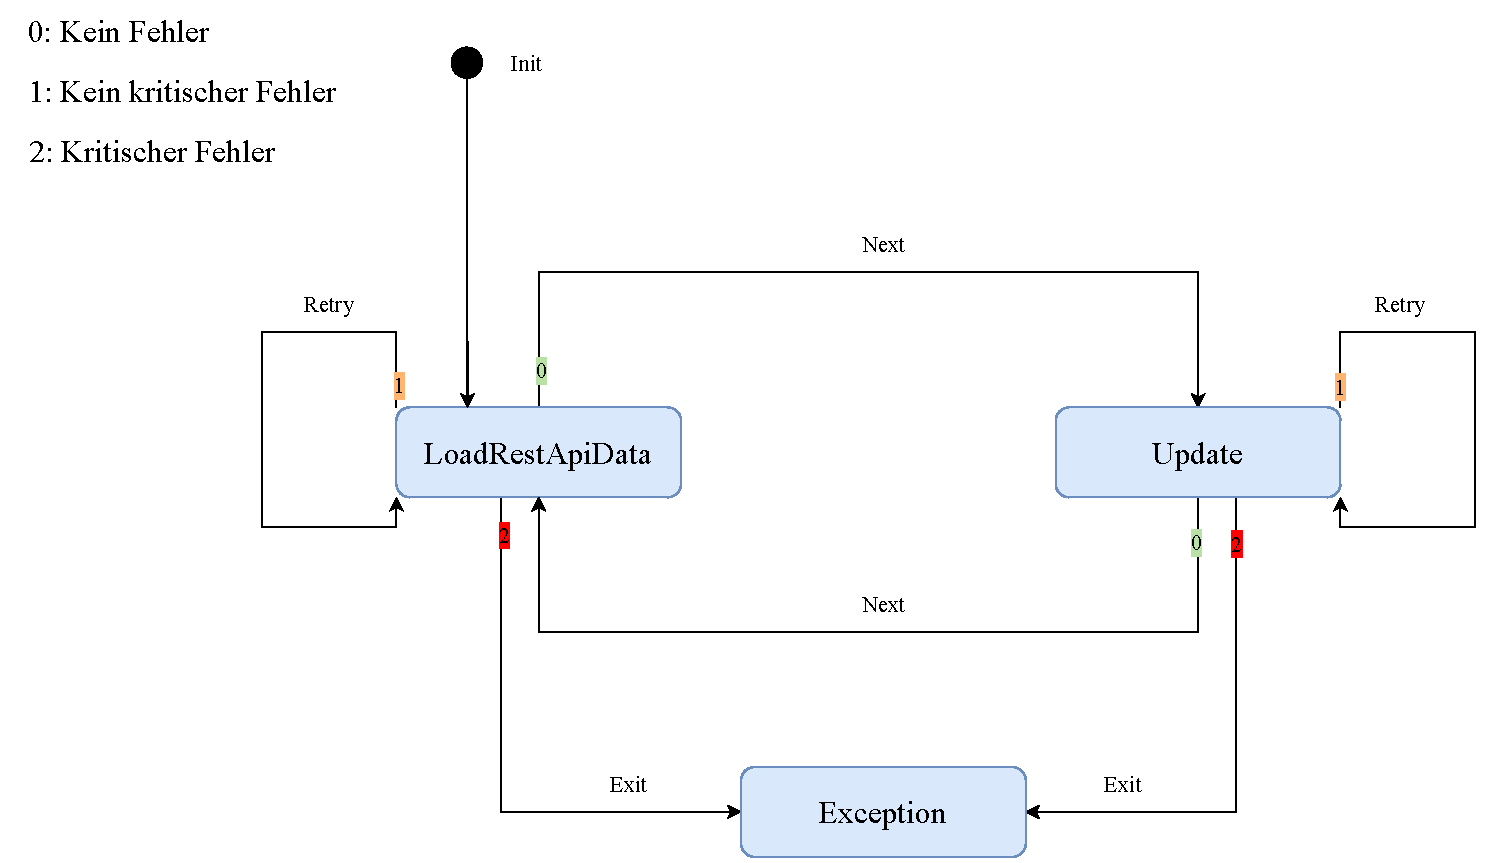
\includegraphics[width=\linewidth]{figures/statemachine.pdf}
    \caption{Zustandsmaschine des Imports}
    \label{fig:statemachine}
\end{figure}
\subsection{Fehlerbehandlung}
Die Fehlerbehandlung lässt sich in zwei Kategorien unterteilen. Zum einen das Erkennen oder Abfangen der Fehler und zum anderen das Dokumentieren und Erfassen der Herkunft und Gründe.
Das Abfangen der Fehler erfolgt durch gezieltes Ausnahmebehandlungen in der Software, zum Beispiel bei der Verbindung an die Datenbank, und den in Kapitel \ref{sec-zustandsmaschine} angesprochenen Überprüfungen der Sinnhaftigkeit
von den gelieferten Daten. Für die zweite Kategorie wird durch Logs und Metadaten die Nachvollziehbarkeit der Fehler sichergestellt.
\subsubsection{Logs}
In der Software wurde sich für das Paket \textit{Serilog} entschieden, da es eine einfache Möglichkeit bietet, Log-Dateien zu verwalten.
Der Hauptnutzen dieser Dateien liegt in der Dokumentation der Fehlerart und Fehlerstelle. Sollte zum Beispiel die Verbindung zu der Datenbank
unterbrochen werden und eine Ausnahme wird ausgelöst, dann wird der Fehler, der Zeitpunkt, die Klasse und die Methode in eine Datei geschrieben.
Dieses erfordert außerdem einige Anpassungen an das Dockersystem. Damit die Log-Dateien auch persistent sind, wurde ein Volume genutzt, welches auf einen
entsprechenden Speicherort gemountet wird.
\subsubsection{Metadaten des Imports}
\label{sec-metadata-import}
Die Metadaten befassen sich mit dem zusätzlichen Speichern von Daten über den Import und dem Verändern der Daten seitens des Datenbanksystems.
An jede Relation werden die Attribute \textit{UPDATE\_NAME}, \textit{UPDATE\_TS}, \textit{INSERT\_NAME}, \textit{INSERT\_TS} angehangen.
In den Spalten \textit{INSERT\_NAME}, \textit{INSERT\_TS} wird festgehalten, welche Maschine/Nutzer zu welchem Zeitpunkt die Daten eingepflegt hat. In den anderen beiden
Spalten werden bei allen Änderungen der Daten in der Tabelle der Nutzer/Maschine und der Zeitpunkt erfasst. Beim ersten Hinzufügen der Daten sind \textit{INSERT\_NAME} und \textit{UPDATE\_NAME}, bzw.
\textit{INSERT\_TS} und \textit{UPDATE\_TS} identisch.\\
Sowohl durch die Logs als auch durch die eben beschriebenen Metadaten wird noch keine Nachvollziehbarkeit der importierten Daten geliefert.
Wird durch eine Überprüfung der importierten Daten festgestellt, dass ein Fehler aufgetreten ist, dann lässt sich nur schwer zurückverfolgen, ob die Software falsch programmiert worden ist
oder sich die gelieferte Datenstruktur geändert hat. Des Weiteren lassen sich die fehlerhaften Daten im Nachhinein nicht korrigieren. Um diese Punkte
zu behandeln gibt es eine weitere Relation \textit{TBL\_IMPORT}. Diese wird beim Importieren der Daten selber mit einer \textit{IDNR} und einem Zeitstempel versehen. Außerdem wird der komplette JSON-String als Bytearray in der Spalte \textit{RAWDATA}
gespeichert. Zusätzlich erhält jede andere Relation ein Attribut \textit{IMPORT\_FOREIGN\_KEY}, welches ein Fremdschlüssel auf die \textit{IDNR} in der Tabelle \textit{TBL\_IMPORT} ist. Dadurch lässt sich nachvollziehen, wann der Import mit welcher JSON
stattgefunden hat und durch den JSON-String selber können Fehler im Nachhinein angepasst werden. 

